% -*- root: 00-main.tex -*-
\section*{Results}
\label{sec:results}

\subsection*{Proof of concept on digital phantoms}
\label{sec:results_phantom}
Using the experimental instrumentation described in section \nameref{sec:experiments_evaluation},
  we collected quantitative results on the digital phantoms.
To warp the simulated datasets, we generated 150 realizations of random and smooth displacement
  fields $U^{-1}_{true}$.
Smoothness is achieved using two levels of B-Spline functions, with control points evenly
  located in isotropic grids covering the full extent of the phantom.
The first level had $50.5mm$ of separation between control points and the second $25.25mm$.
The rationale behind this choice is producing large deformations on the contours with
  the first level, and matching the properties of susceptibility-derived distortions
  as previously reported by \cite{irfanoglu_susceptibility_2011} with the finer grid.
Invertibility of $U^{-1}_{true}$ is ensured by controlling the maximum displacement at each
  level ($20.2mm$ and $10.1mm$ respectively) as studied in \citep{rueckert_diffeomorphic_2006}.

A total of 1200 registration experiments (4 phantom types $\times$ 150 random warpings
  $\times$ 2 resolutions) were run.
For each registration, the averaged Hausdorff distance (see \nameref{sec:experiments_evaluation})
  of the inner and the outer surfaces was computed.
The results showed a consistent and high accuracy, below voxel resolution.
\autoref{fig:phantom} (block C) presents the box plots by model type corresponding
  to the two sets of resolutions of generated phantoms.
To support that the missregistration errors averaged per experiment was significantly
  under the resolution of the target image, we proceeded as follows.
First, we confirmed that the error distributions were skewed using a Shapiro-Wilk test of
  normality.
All the distributions of errors under test (4 phantom types $\times$ 2 resolutions) resulted
  non-normal with $p<0.001$.
Consequently, we used the non-parametric Wilcoxon signed-rank test along with Bonferroni
  correction for multiple comparisons ($N=150$).
Averaged errors resulted significantly lower than voxel resolution with $p < (0.001 / 150)$
  for all the tests (4 phantom types $\times$ 2 resolutions).

\subsection*{Correction of distortions on real datasets}\label{sec:results_hcp}

\paragraph*{Assessing the segmentation model}\label{sec:res_model_and_metric} %
%
Preliminarly, we investigated the aptness of our segmentation model to play as cost function
  driving the registration process.
First, we selected the 6-regions model described in \nameref{sec:human_connectome} after
  visual evaluation of the joint distribution {\color{red} REF Supplemental} of several
  alternative models for segmenting the target bivariate images (\gls*{fa} and \gls*{adc}).
Since susceptibility-derived distortions are always aligned with the phase encoding axis
  and feature the property of being linear with respect to the phase inhomogeneity map,
  we reduced the dimensionality of the error space to one dimension.
Thus, the energy functional \eqref{eq:energy} was evaluated for the contour positions
  obtained along a lineralized space of distortions
  $\hat{U}\{\vec{r}\} = \epsilon \cdot U_{true} = \vec{r} + \epsilon \cdot u(\vec{r})$,
  with $\epsilon \in [-1.1, 1.1]$.
The result of this experiment is shown in \autoref{fig:energymap}.
The metric consistently displayed its minimum at the zero-error point.

\begin{figure}
	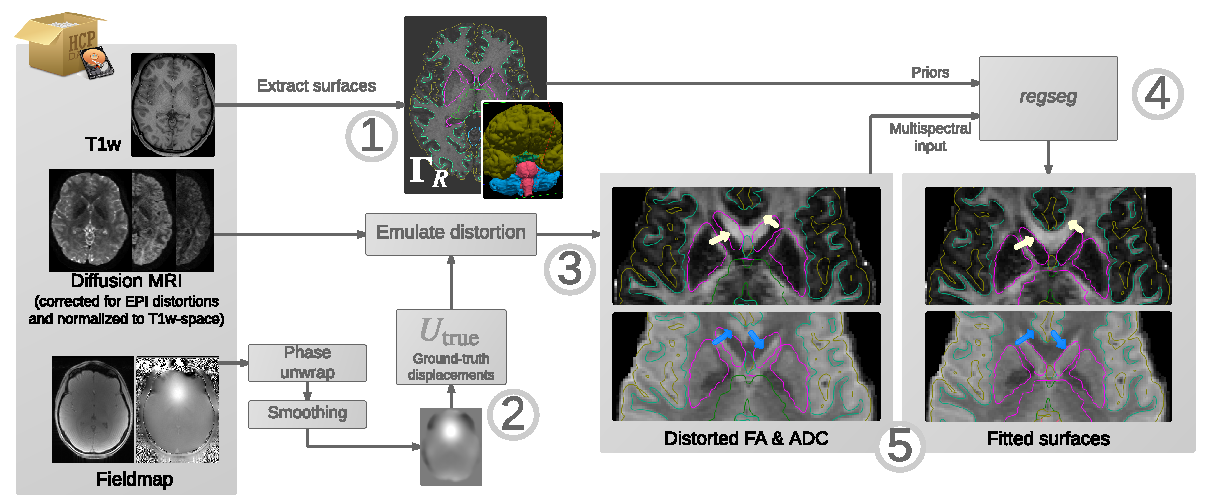
\includegraphics[width=\linewidth]{figures/figure04.pdf}
	\caption{Assessment of the segmentation model, sampling the value of the energy functional
	\eqref{eq:energy} versus several registration errors generated as explained in
	\nameref{sec:res_model_and_metric}.
	The metric of our registration method displayed a smooth gradient towards the minimum
	located at the $\epsilon = 0.0$ point.}\label{fig:energymap}
\end{figure}

\paragraph*{Cross-comparison evaluation}\label{sec:res_cc_evaluation}
%
Finally, we evaluated the performance of our registration method, and compared it to correcting
  for distortions using the \emph{b0}-to-\gls*{t2} registration approach.